\documentclass[11pt,a4paper]{article}

\usepackage[utf8]{inputenc}
\usepackage[T1]{fontenc}
\usepackage{lmodern}
\usepackage[margin=2.4cm]{geometry}
\usepackage{amsmath,amssymb}
\usepackage{graphicx}
\usepackage{booktabs}
\usepackage{array}
\usepackage{longtable}
\usepackage{enumitem}
\usepackage{caption}
\usepackage{float}
\usepackage{microtype}
\usepackage{hyperref}
\usepackage{siunitx}
\usepackage{xcolor}
\usepackage{fancyhdr}

\hypersetup{colorlinks=true,linkcolor=black,urlcolor=blue,citecolor=black}
\sisetup{per-mode=symbol,detect-all,exponent-product=\times}

\pagestyle{fancy}
\fancyhf{}
\lhead{Les sylphes -- updated checked solution}
\rhead{TLE exam}
\cfoot{\thepage}

\setlength{\headheight}{14pt}
\setlength{\parindent}{0pt}
\setlength{\parskip}{0.55em}
\renewcommand{\arraystretch}{1.18}

\newenvironment{finalanswer}{%
  \begin{center}\begin{minipage}{0.94\linewidth}\hrule\vspace{0.45em}\textbf{Final answer. }%
}{%
  \vspace{0.45em}\hrule\end{minipage}\end{center}%
}

\newcommand{\E}{\mathbf{E}}
\newcommand{\B}{\mathbf{B}}
\newcommand{\jv}{\mathbf{j}}
\newcommand{\grad}{\operatorname{grad}}
\newcommand{\RT}{R_T}
\newcommand{\gzero}{g_0}
\newcommand{\ISS}{\mathrm{ISS}}
\newcommand{\Otwo}{\ensuremath{\mathrm{O}_2}}
\newcommand{\Ntwo}{\ensuremath{\mathrm{N}_2}}
\newcommand{\eV}{\ensuremath{\mathrm{eV}}}

\title{Concours Commun Mines-Ponts (CCMP) 2023\\[0.25em]
\large Physics I Exam, PC Track\\[0.8em]
\Large Les sylphes\\[0.25em]
\large Updated Checked Solution}
\author{}
\date{}

\begin{document}
\maketitle

\tableofcontents
\newpage

\section*{Checked answer key}
\addcontentsline{toc}{section}{Checked answer key}

\begin{longtable}{>{\raggedright\arraybackslash}p{0.12\linewidth}>{\raggedright\arraybackslash}p{0.80\linewidth}}
\toprule
\textbf{Question} & \textbf{Main checked result}\\
\midrule
1 & Sprites are red because the emission spectrum is strongest in the red / near infrared. Ground observation is hard because the downward path crosses absorbing atmosphere, especially the oxygen band near \SI{762}{nm}.\\
2 & Pic du Midi to the French Alps is of order \SI{500}{km}; using a somewhat larger Mont Blanc distance, around \SI{600}{km}, would give a horizon height closer to \SI{30}{km}. In either case, sprites at \SIrange{40}{80}{km} can clear the horizon, while Mont Blanc cannot in the no-refraction model.\\
3 & The same localized signal appears in visible and in the \SI{761}{nm} filtered image. A normal lightning flash would give a filtered/visible ratio $30/836\simeq3.6\times10^{-2}$, whereas the event has a much stronger relative narrow-band signal: this supports a sprite detection.\\
4--6 & At \SI{400}{km}: $G_{\ISS}\simeq \SI{9}{m.s^{-2}}$, $v_{\ISS}\simeq \SI{8}{km.s^{-1}}$, $T_{\ISS}\simeq \SI{90}{min}$.\\
7 & A \SI{20}{km} camera field is crossed in about \SI{2.5}{s}. A sprite lasting a few \SI{0.1}{s} can be recorded, with roughly kilometre-scale precision.\\
8--12 & Hydrostatic model gives $H=RT_0/(Mg_0)\simeq \SI{9}{km}$ and the pressure law in the statement. The model fails mainly because the assumed linear temperature law is unrealistic above the troposphere.\\
13--16 & Collisionless plasma: $\gamma_p=-i n e^2/(m_e\omega)$, $\omega^2=\omega_p^2+c^2k^2$, and for $n=10^{11}\,\mathrm{m^{-3}}$, $f_p\simeq\SI{3}{MHz}$.\\
17 & A \SI{2.2}{MHz} radar reflects where $f_p\geq\SI{2.2}{MHz}$, i.e. $n_e\gtrsim \SI{6e10}{m^{-3}}$. The transient radar columns are consistent with sprite-related ionization.\\
18--20 & $N(x)=N_0\exp(-n_{\rm mol}S_{\rm eff}x)$, $\ell_{pm}=1/(n_{\rm mol}S_{\rm eff})$, and at \SI{60}{km}, $\ell_{pm}\simeq\SI{2}{cm}$.\\
21--24 & A resting electron gains only about \SI{2}{eV} over one mean free path in a \SI{100}{V.m^{-1}} field. A \SI{1}{MeV} electron is relativistic. The avalanche stage number is $\mathcal{N}\simeq35$, i.e. order $4\times10^1$.\\
\bottomrule
\end{longtable}

\section{Extracted figures}

These are the figures used in the reasoning below. They are included so the LaTeX file can be read without switching back to the exam statement.

\begin{figure}[H]
\centering
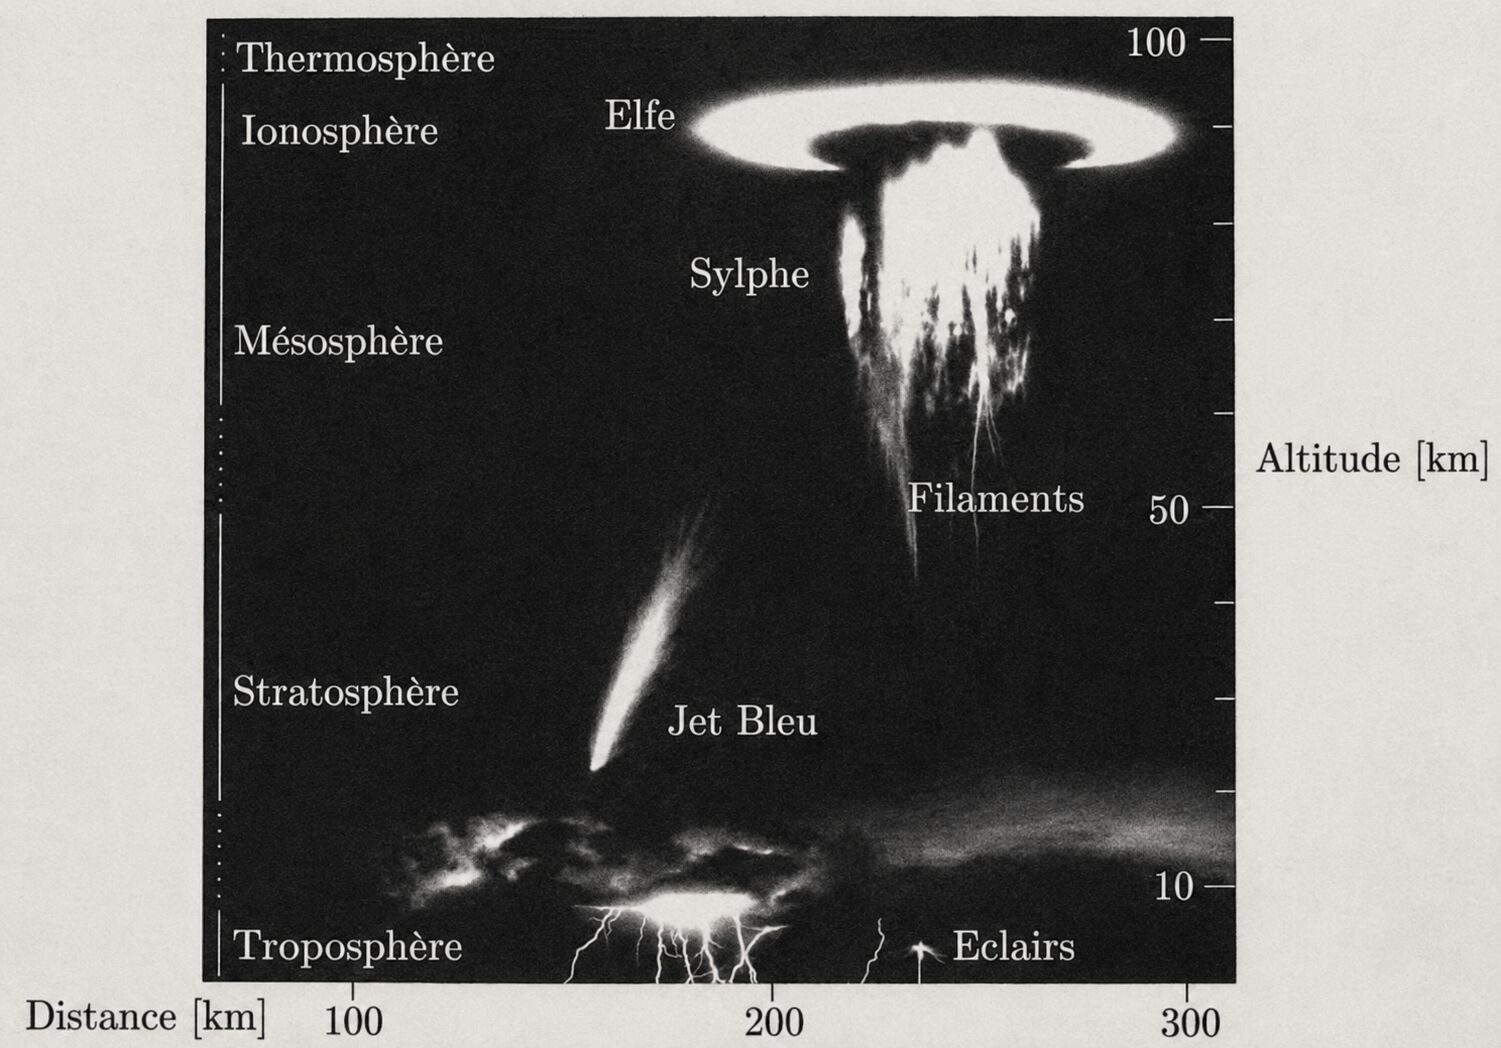
\includegraphics[width=0.72\linewidth]{figures_compressed/figure_01.jpg}
\caption{Figure 1: atmospheric luminous events and altitude scale.}
\end{figure}

\begin{figure}[H]
\centering
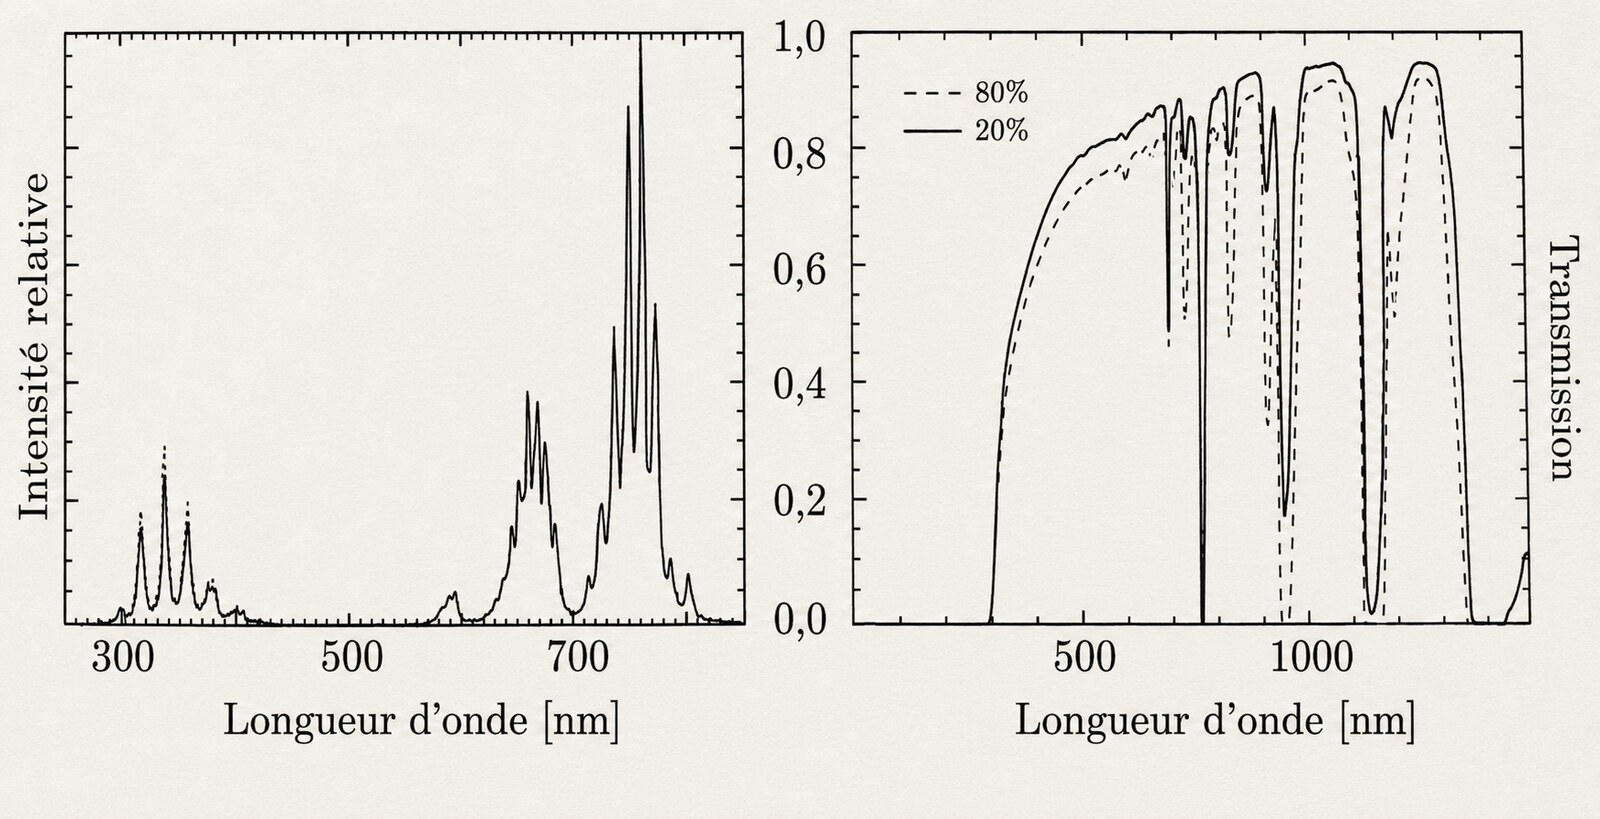
\includegraphics[width=0.94\linewidth]{figures_compressed/figure_02.jpg}
\caption{Figure 2: sprite emission spectrum and atmospheric transmission.}
\end{figure}

\begin{figure}[H]
\centering
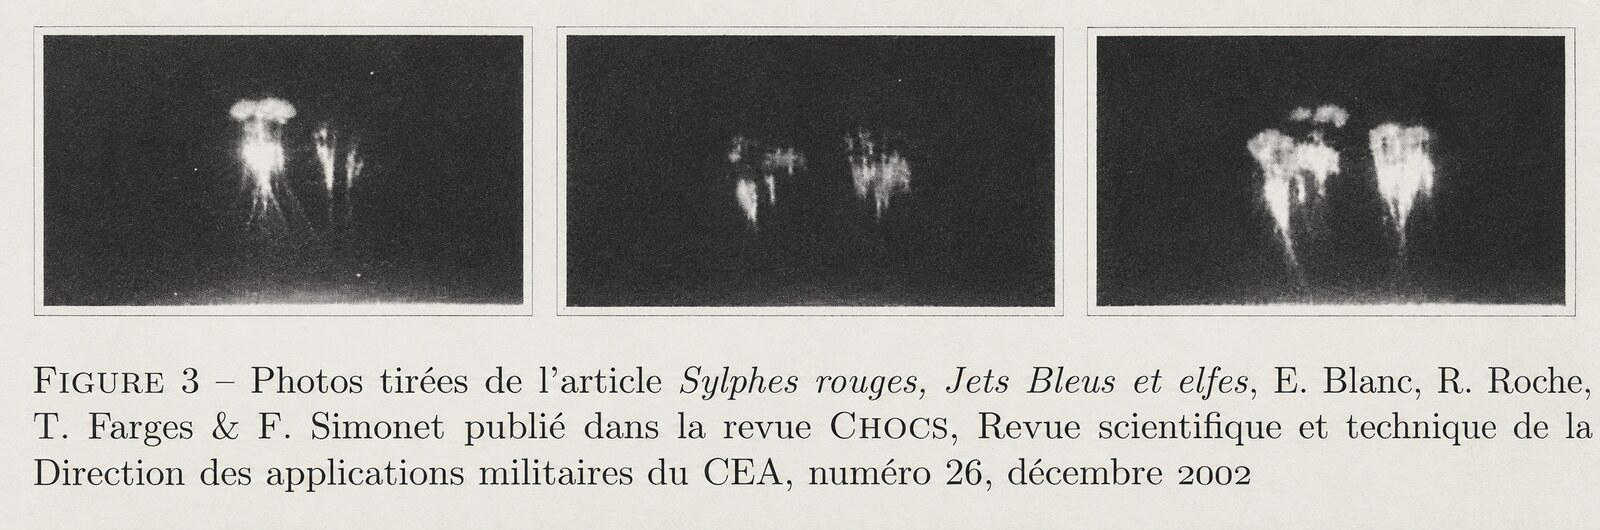
\includegraphics[width=0.86\linewidth]{figures_compressed/figure_03.jpg}
\caption{Figure 3: sprite photographs taken from Pic du Midi.}
\end{figure}

\begin{figure}[H]
\centering
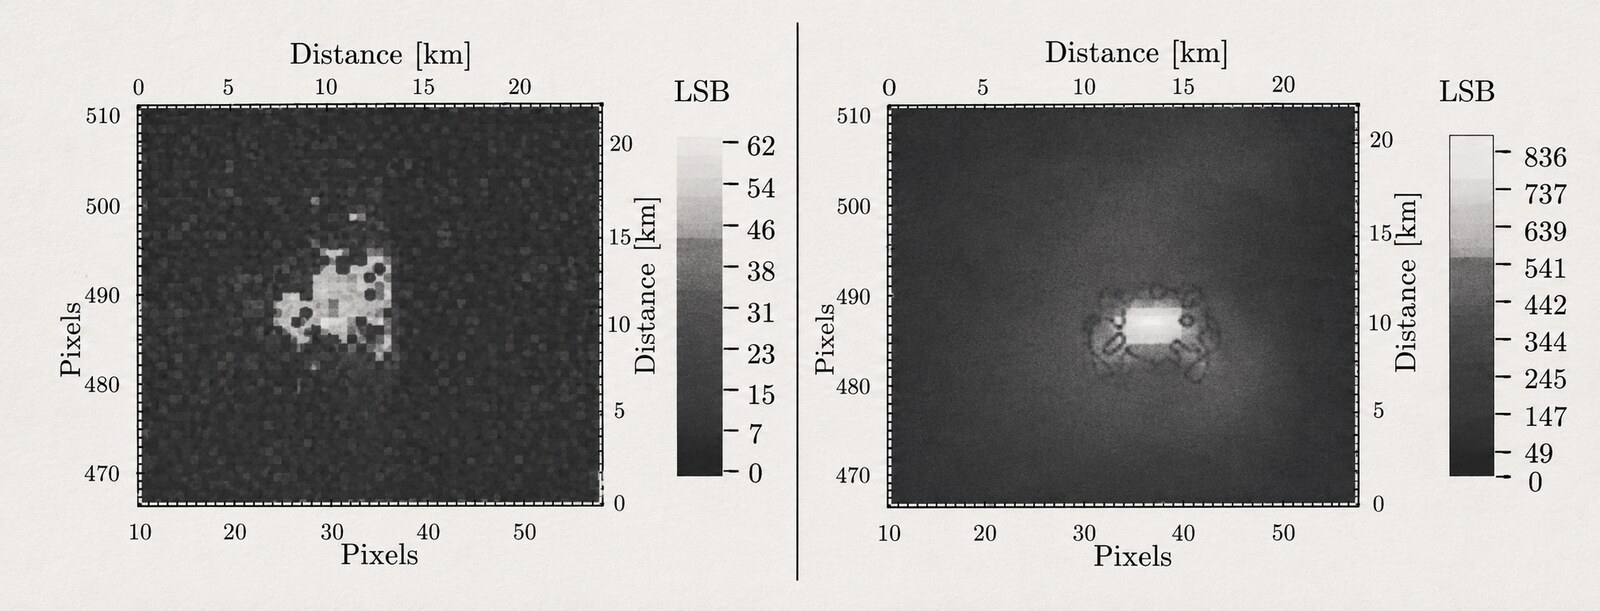
\includegraphics[width=0.94\linewidth]{figures_compressed/figure_04.jpg}
\caption{Figure 4: ISS filtered and visible microcamera images.}
\end{figure}

\begin{figure}[H]
\centering
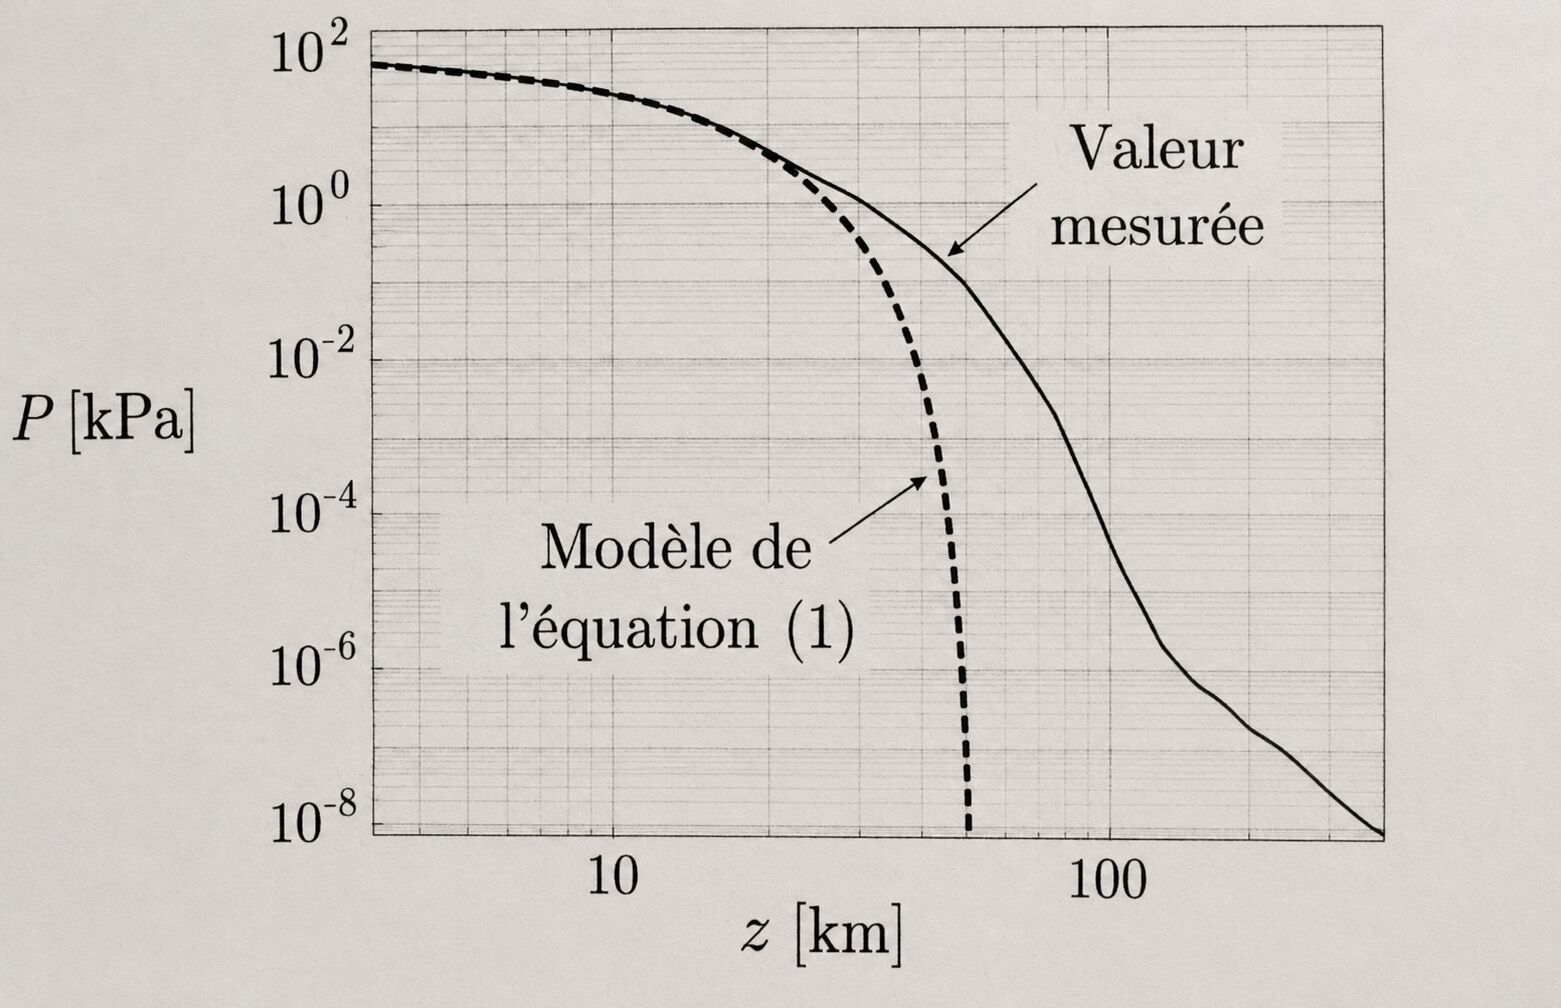
\includegraphics[width=0.72\linewidth]{figures_compressed/figure_05.jpg}
\caption{Figure 5: atmospheric pressure model compared with measured pressure.}
\end{figure}

\begin{figure}[H]
\centering
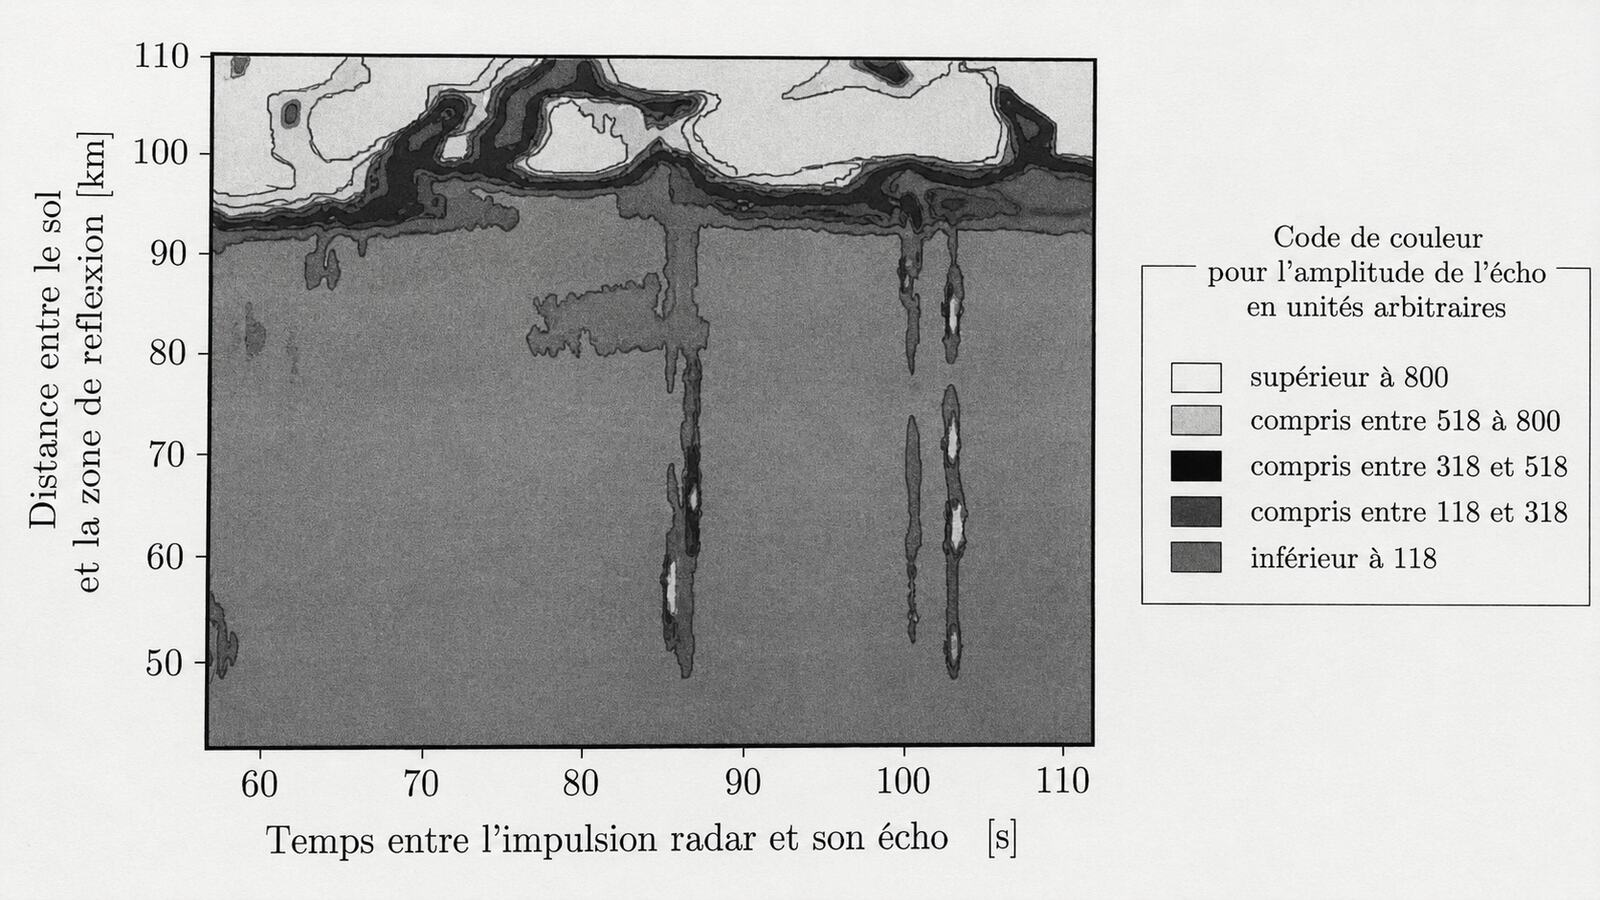
\includegraphics[width=0.86\linewidth]{figures_compressed/figure_06.jpg}
\caption{Figure 6: radar echo map at \SI{2.2}{MHz}.}
\end{figure}

\begin{figure}[H]
\centering
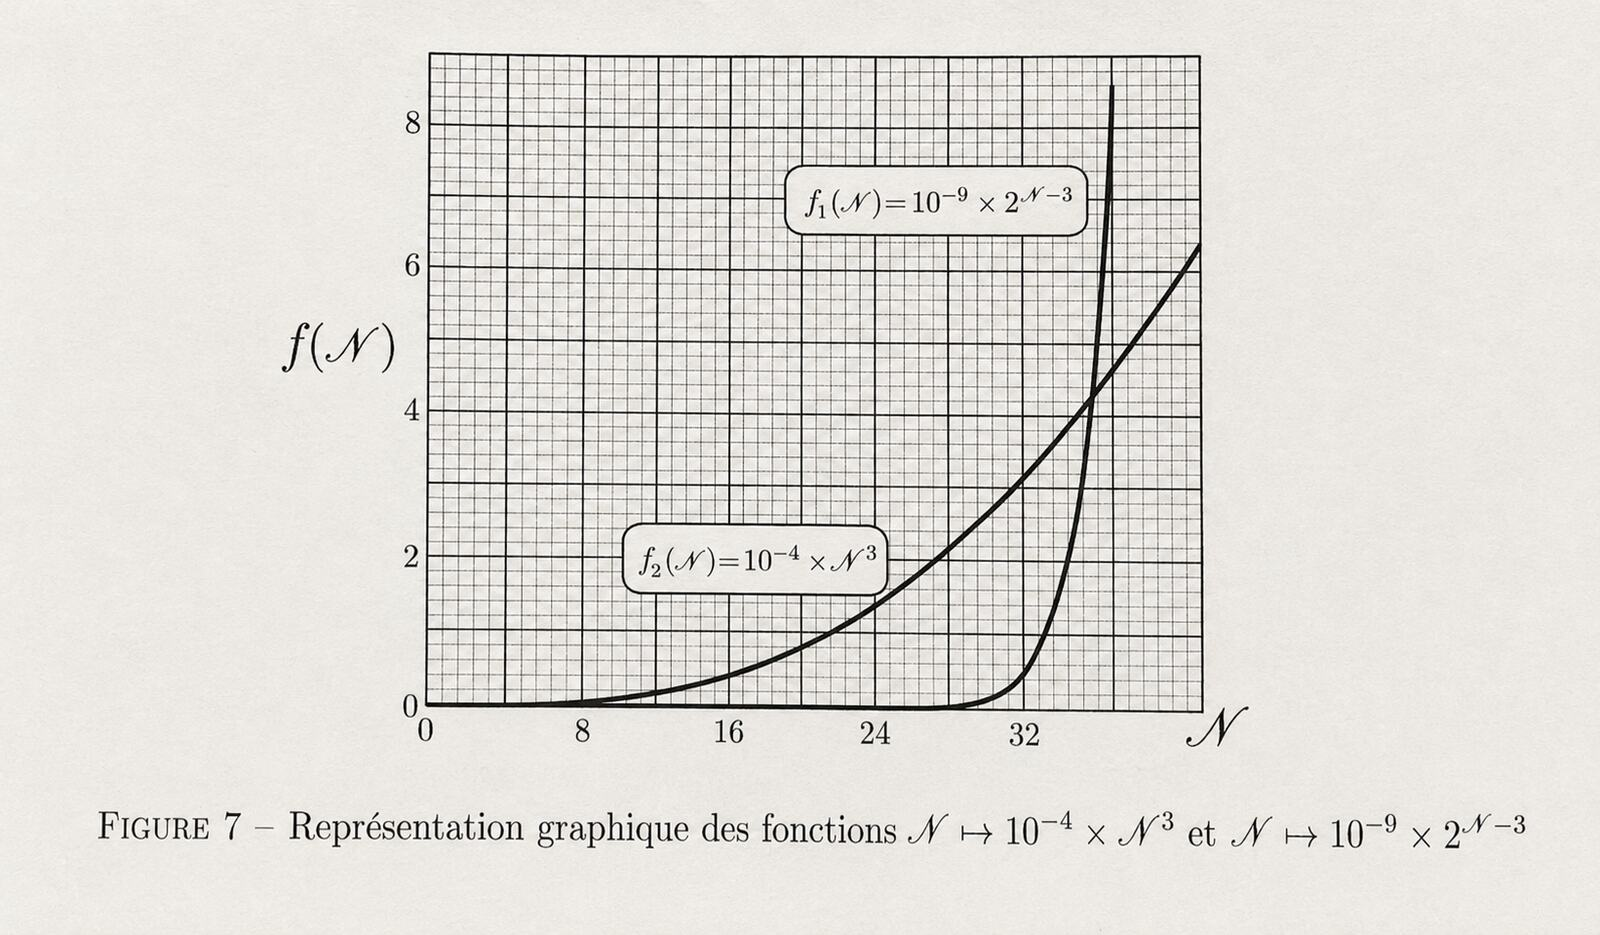
\includegraphics[width=0.82\linewidth]{figures_compressed/figure_07.jpg}
\caption{Figure 7: graphical solution for the avalanche stage count.}
\end{figure}

\newpage
\section{Observation des sylphes}

\subsection*{Question 1 -- Colour and why ground observation is difficult}
\addcontentsline{toc}{subsection}{Question 1}

The left graph in Figure 2 is an emission spectrum. The largest peaks are mostly between about \SI{600}{nm} and \SI{800}{nm}. This is the red and near-infrared region of the spectrum. That is why sprites, or ``sylphes'', have a red colour.

The right graph in Figure 2 shows atmospheric transmission for light emitted from a source at about \SI{80}{km} altitude and detected from the ground. A transmission near 1 means the light passes through the atmosphere well; a transmission near 0 means the atmosphere absorbs it strongly. The curve has deep absorption dips, especially in the near infrared. The statement later points out the oxygen absorption band around \SI{762}{nm}, very close to the sprite emission region. Water vapour also causes absorption, and the result depends on humidity.

So there are three reasons ground observation is difficult:
\begin{enumerate}[label=\arabic*)]
\item sprites are brief, lasting only a few hundred milliseconds;
\item they are far away and high in the atmosphere;
\item part of their red / near-infrared light is absorbed before reaching the ground.
\end{enumerate}

\begin{finalanswer}
Sprites appear red because their strongest emission lies in the red / near-infrared. They are hard to observe from the ground because they are short-lived and because atmospheric absorption, especially near \SI{762}{nm}, removes part of their light.
\end{finalanswer}

\subsection*{Question 2 -- Earth curvature and visibility from Pic du Midi}
\addcontentsline{toc}{subsection}{Question 2}

The Pic du Midi is in the Pyrenees. The French Alps and Mont Blanc are several hundred kilometres away. Among \SI{500}{km}, \SI{1000}{km}, and \SI{1500}{km}, the correct order of magnitude for the exam is therefore
\[
 d\sim\SI{500}{km}.
\]
A more precise distance to a specific Alpine target such as Mont Blanc can be closer to about \SI{600}{km}. This does not change the conclusion; it only raises the geometric horizon estimate from about \SI{20}{km} to about \SI{30}{km}.

Now ignore the altitude of Pic du Midi, as requested. The observer is placed on the surface of a spherical Earth. The line of sight to the horizon is tangent to Earth. A point at distance $d$ along Earth's surface is hidden below the tangent line by a height $h$.

Let $\theta=d/\RT$. From the right triangle formed by Earth's centre, the observer, and the point above the horizon,
\[
 \cos\theta=\frac{\RT}{\RT+h}.
\]
Therefore
\[
 h=\RT\left(\frac{1}{\cos(d/\RT)}-1\right).
\]
For $d\ll \RT$, use $\cos\theta\simeq1-\theta^2/2$, so
\[
 h\simeq \frac{d^2}{2\RT}.
\]
With $d=\SI{500}{km}$ and $\RT=\SI{6400}{km}$,
\[
 h\simeq \frac{(\SI{5.0e5}{m})^2}{2\times \SI{6.4e6}{m}}
      \simeq \SI{2.0e4}{m}
      \simeq \SI{20}{km}.
\]

Sprites lie roughly between \SI{40}{km} and \SI{80}{km}, so they can be above this geometric horizon. Mont Blanc is only about \SI{4.8}{km} high, which is far below even the \SIrange{20}{30}{km} horizon-height estimate. In the no-refraction model, Mont Blanc is not visible from Pic du Midi at this distance.

\begin{finalanswer}
$d\sim\SI{500}{km}$ for the exam order of magnitude, giving $h\sim\SI{20}{km}$. A \SI{600}{km} distance would give $h\sim\SI{30}{km}$. Alpine sprites can be visible because they are much higher than this, but Mont Blanc cannot be seen in this simplified no-refraction geometry.
\end{finalanswer}

\subsection*{Question 3 -- Why Figure 4 proves a sprite detection}
\addcontentsline{toc}{subsection}{Question 3}

Figure 4 compares two simultaneous ISS images: a narrow-band image filtered around \SI{761}{nm} and a visible-light image. The statement gives a useful calibration: a normal lightning flash gives about 836 LSB in the visible camera but only about 30 LSB in the filtered camera. For ordinary lightning, the filtered/visible ratio is therefore only
\[
 \frac{30}{836}\simeq3.6\times10^{-2}.
\]

In the event shown, the same localized object appears in the two images, at the same place. The filtered image has a clear signal in the narrow band associated with sprite emissions. Reading the colour bars only approximately, the filtered image reaches tens of LSB while the visible image reaches a few hundred LSB, so the relative narrow-band signal is much larger than the ordinary-lightning calibration ratio. This is important because random noise would not appear at the same position in both cameras, and ordinary lightning would not be expected to give such a strong narrow-band signature.

\begin{finalanswer}
The co-located visible and \SI{761}{nm} signals identify the same luminous event, and the filtered/visible ratio is much larger than the $30/836\simeq0.036$ ordinary-lightning calibration. This supports the detection of a sprite.
\end{finalanswer}

\subsection*{Question 4 -- Gravity at ISS altitude}
\addcontentsline{toc}{subsection}{Question 4}

The ISS is at altitude $h_{\ISS}\simeq\SI{400}{km}$. Outside a spherically symmetric Earth, Gauss' theorem tells us that the gravitational field is the same as if all of Earth's mass were concentrated at its centre.

At Earth's surface,
\[
 g_0=\frac{G M_T}{\RT^2}.
\]
At ISS altitude,
\[
 G_{\ISS}=\frac{G M_T}{(\RT+h_{\ISS})^2}.
\]
Divide the second equation by the first:
\[
 G_{\ISS}=g_0\left(\frac{\RT}{\RT+h_{\ISS}}\right)^2
          =g_0\left(1+\frac{h_{\ISS}}{\RT}\right)^{-2}.
\]
Numerically,
\[
 \frac{h_{\ISS}}{\RT}=\frac{400}{6400}=0.0625,
\]
so
\[
 G_{\ISS}=\frac{9.8}{(1.0625)^2}\simeq\SI{8.7}{m.s^{-2}}.
\]

\begin{finalanswer}
\[
G_{\ISS}=g_0\left(1+\frac{h_{\ISS}}{\RT}\right)^{-2}\simeq\SI{9}{m.s^{-2}}.
\]
\end{finalanswer}

\subsection*{Question 5 -- ISS orbital speed}
\addcontentsline{toc}{subsection}{Question 5}

For a circular orbit, the speed is constant in magnitude, but the velocity direction changes. The required centripetal acceleration is
\[
 a_c=\frac{v_{\ISS}^2}{\RT+h_{\ISS}}.
\]
Gravity provides this acceleration, so
\[
 \frac{v_{\ISS}^2}{\RT+h_{\ISS}}=G_{\ISS}.
\]
Thus
\[
 v_{\ISS}=\sqrt{G_{\ISS}(\RT+h_{\ISS})}.
\]
Using the expression from Question 4,
\[
 v_{\ISS}=\sqrt{\frac{g_0\RT^2}{\RT+h_{\ISS}}}.
\]
Numerically,
\[
 v_{\ISS}\simeq\sqrt{\frac{9.8(\SI{6.4e6}{m})^2}{\SI{6.8e6}{m}}}
 \simeq \SI{7.7e3}{m.s^{-1}}.
\]

\begin{finalanswer}
\[
v_{\ISS}\simeq\SI{8}{km.s^{-1}}.
\]
\end{finalanswer}

\subsection*{Question 6 -- ISS period and Kepler's third law}
\addcontentsline{toc}{subsection}{Question 6}

One circular orbit has length $2\pi(\RT+h_{\ISS})$. Therefore
\[
 T_{\ISS}=\frac{2\pi(\RT+h_{\ISS})}{v_{\ISS}}.
\]
Substitute the speed from Question 5:
\[
 T_{\ISS}=2\pi\sqrt{\frac{(\RT+h_{\ISS})^3}{g_0\RT^2}}.
\]
Since $g_0\RT^2=G M_T$, this is also
\[
 T_{\ISS}=2\pi\sqrt{\frac{r^3}{G M_T}},\qquad r=\RT+h_{\ISS}.
\]
Squaring,
\[
 T_{\ISS}^2=\frac{4\pi^2}{G M_T}r^3.
\]
This is Kepler's third law: $T^2$ is proportional to $r^3$.

Numerically,
\[
 T_{\ISS}\simeq \frac{2\pi(\SI{6.8e6}{m})}{\SI{7.7e3}{m.s^{-1}}}
 \simeq\SI{5.6e3}{s}
 \simeq\SI{93}{min}.
\]

\begin{finalanswer}
\[
T_{\ISS}\simeq\SI{90}{min},\qquad T^2\propto r^3.
\]
\end{finalanswer}

\subsection*{Question 7 -- Can the ISS cameras record a whole sprite?}
\addcontentsline{toc}{subsection}{Question 7}

Figure 4 has a field of view of about \SI{20}{km} by \SI{20}{km}. With $v_{\ISS}\simeq\SI{8}{km.s^{-1}}$, the time for the ISS ground track to cross \SI{20}{km} is
\[
 \Delta t_{\rm field}\simeq \frac{\SI{20}{km}}{\SI{8}{km.s^{-1}}}\simeq\SI{2.5}{s}.
\]
A sprite lasts only a few hundred milliseconds. For example,
\[
\SI{0.1}{s}\Rightarrow \Delta x\simeq\SI{0.8}{km},
\qquad
\SI{0.3}{s}\Rightarrow \Delta x\simeq\SI{2.4}{km}.
\]
These distances are much smaller than the \SI{20}{km} field of view, so recording the whole event is possible if the storm lies inside the field at the right time.

For precision, the image scale is roughly
\[
 \frac{\SI{20}{km}}{40\text{--}50\text{ pixels}}\simeq \SIrange{0.4}{0.5}{km/pixel}.
\]
The ISS also moves by about a kilometre during a typical event. So the natural spatial precision is not metres; it is about a kilometre.

\begin{finalanswer}
Recording a whole sprite is possible: the field is crossed in about \SI{2.5}{s}, while the sprite lasts only a few \SI{0.1}{s}. The spatial precision is roughly kilometre-scale because of the pixel size and ISS motion.
\end{finalanswer}

\section{Une atmosph\`ere \`a pression variable}

\subsection*{Question 8 -- Hydrostatic equation and scale height}
\addcontentsline{toc}{subsection}{Question 8}

The vector law of hydrostatic equilibrium is
\[
 \grad P=\mu\,\mathbf{g},
\]
where $\mu$ is the mass density and $\mathbf{g}$ points downward. If $z$ is upward, this becomes
\[
 \frac{dP}{dz}=-\mu g(z).
\]

The atmosphere is treated as an ideal gas. For molar mass $M$,
\[
 \mu=\frac{PM}{RT(z)}.
\]
The temperature model is
\[
 T(z)=T_0\left(1-\frac{z}{\ell}\right),
\]
and gravity is
\[
 g(z)=g_0\left(1+\frac{z}{\RT}\right)^{-2}.
\]
Therefore
\[
 \frac{dP}{dz}
 =-\frac{PM}{RT_0(1-z/\ell)}g_0\left(1+\frac{z}{\RT}\right)^{-2}.
\]
Define the characteristic height
\[
 H=\frac{RT_0}{Mg_0}.
\]
Then
\[
 \frac{dP}{dz}=-F(z)\frac{P}{H},
 \qquad
 F(z)=\frac{1}{(1-z/\ell)(1+z/\RT)^2}.
\]

Numerically, with $T_0=\SI{290}{K}$ and $M=\SI{29e-3}{kg.mol^{-1}}$,
\[
 H=\frac{8.31\times 290}{0.029\times9.8}\simeq\SI{8.5e3}{m}\simeq\SI{9}{km}.
\]

\begin{finalanswer}
\[
\frac{dP}{dz}=-F(z)\frac{P}{H},\qquad
F(z)=\frac{1}{(1-z/\ell)(1+z/\RT)^2},\qquad
H=\frac{RT_0}{Mg_0}\simeq\SI{9}{km}.
\]
\end{finalanswer}

\subsection*{Question 9 -- Pressure law}
\addcontentsline{toc}{subsection}{Question 9}

The statement gives a decomposition
\[
F(z)=\frac{\alpha}{1-z/\ell}+\frac{\beta+\gamma z}{(1+z/\RT)^2},
\]
with $\varepsilon=\ell/\RT$. Since
\[
 \varepsilon=\frac{50}{6400}\simeq 8\times10^{-3}\ll1,
\]
we may use
\[
\alpha\simeq1,
\qquad
\beta\simeq2\varepsilon,
\qquad
\gamma\simeq\frac{\varepsilon}{\RT}.
\]

The pressure equation is
\[
 \frac{dP}{P}=-\frac{F(z)}{H}\,dz.
\]
Integrate from $0$ to $z$, using $P(0)=P_0$.

First term:
\[
 \int_0^z \frac{du}{1-u/\ell}
 =-\ell\ln\left(1-\frac{z}{\ell}\right).
\]
This gives the factor
\[
 \left(1-\frac{z}{\ell}\right)^{\ell/H}.
\]

For the second term, with $y=1+u/\RT$, one obtains
\[
\int_0^z \frac{2\varepsilon+(\varepsilon/\RT)u}{(1+u/\RT)^2}\,du
=\ell\left[\ln\left(1+\frac{z}{\RT}\right)+1-\frac{1}{1+z/\RT}\right].
\]
Here we used $\varepsilon\RT=\ell$. Also,
\[
1-\frac{1}{1+z/\RT}=\frac{z/\RT}{1+z/\RT}.
\]
So, after multiplication by $-1/H$, the non-logarithmic part contributes
\[
-\frac{\ell}{H}\frac{z/\RT}{1+z/\RT}
=-\frac{z}{(H\RT/\ell)(1+z/\RT)}.
\]
This gives both a denominator power of $1+z/\RT$ and a small exponential correction.

Thus
\[
P(z)=P_0
\left(\frac{1-z/\ell}{1+z/\RT}\right)^{\xi}
\exp\left[-\frac{z}{\chi(1+z/\RT)}\right],
\]
where
\[
 \xi=\frac{\ell}{H},
 \qquad
 \chi=\frac{H\RT}{\ell}.
\]
Numerically,
\[
 \xi\simeq\frac{50}{8.5}\simeq 5.9\simeq6,
 \qquad
 \chi\simeq\frac{8.5\times6400}{50}\,\si{km}\simeq\SI{1.1e3}{km}.
\]

\begin{finalanswer}
\[
P(z)=P_0
\left(\frac{1-z/\ell}{1+z/\RT}\right)^{\ell/H}
\exp\left[-\frac{z}{(H\RT/\ell)(1+z/\RT)}\right].
\]
So $\xi=\ell/H$ and $\chi=H\RT/\ell$.
\end{finalanswer}

\subsection*{Question 10 -- Useful simplification of the pressure law}
\addcontentsline{toc}{subsection}{Question 10}

For altitudes below \SI{50}{km}, the ratio $z/\RT$ is tiny:
\[
 \frac{50}{6400}\simeq 8\times10^{-3}.
\]
So
\[
 1+\frac{z}{\RT}\simeq 1.
\]
Also $\chi\simeq\SI{1100}{km}$, so
\[
 \exp\left[-\frac{z}{\chi(1+z/\RT)}\right]\simeq 1
\]
for $z\leq\SI{50}{km}$.

Therefore the practical simplified pressure law is
\[
 P(z)\simeq P_0\left(1-\frac{z}{\ell}\right)^{\ell/H}.
\]
This simplification amounts to neglecting the variation of gravity with altitude while keeping the imposed temperature law.

At very low altitude, if $z\ll\ell$, one can go further:
\[
 \left(1-\frac{z}{\ell}\right)^{\ell/H}
 \simeq \exp\left(-\frac{z}{H}\right),
\]
which is the familiar exponential barometric law.

\begin{finalanswer}
\[
P(z)\simeq P_0\left(1-\frac{z}{\ell}\right)^{\ell/H}.
\]
This keeps the temperature decrease but neglects Earth-curvature / gravity variation.
\end{finalanswer}

\subsection*{Question 11 -- Why the model fails near \SI{20}{km}}
\addcontentsline{toc}{subsection}{Question 11}

The model was built with the temperature law
\[
 T(z)=T_0\left(1-\frac{z}{\ell}\right),\qquad \ell=\SI{50}{km}.
\]
This is a simple linear decrease. It is acceptable only as a rough lower-atmosphere model. The real atmosphere does not keep cooling linearly up to \SI{50}{km}: near the tropopause, around \SIrange{10}{20}{km}, the temperature stops following the tropospheric decrease, and in the stratosphere it can even increase.

If the model makes the temperature too low, then the density and pressure decrease too quickly. This matches Figure 5: the model pressure drops away from the measured curve above about \SI{20}{km}.

\begin{finalanswer}
The main failure is the unrealistic linear temperature profile. It stops being valid around the tropopause / lower stratosphere, so the predicted pressure becomes too small above about \SI{20}{km}.
\end{finalanswer}

\subsection*{Question 12 -- Observation from Earth and from the ISS}
\addcontentsline{toc}{subsection}{Question 12}

The oxygen molar fraction is assumed constant:
\[
 x_{\Otwo}\simeq 0.20.
\]
Therefore the oxygen partial pressure is
\[
 P_{\Otwo}(z)=x_{\Otwo}P(z)\simeq0.20P(z).
\]
Near the ground, $P(z)$ is large, so $P_{\Otwo}$ is large. Light travelling downward from a sprite to a ground observer must cross dense oxygen-rich layers. Around \SI{762}{nm}, molecular oxygen absorbs strongly, so the signal can be weakened.

From the ISS, the light path goes upward from the sprite. It avoids most of the dense lower atmosphere. At altitudes of \SIrange{40}{80}{km}, the pressure and oxygen partial pressure are already much smaller than at the ground. Absorption is therefore much weaker for upward observation.

\begin{finalanswer}
Ground observation is difficult because the light crosses dense oxygen-rich air, especially near the \SI{762}{nm} absorption band. ISS observation is easier because the line of sight avoids most of the absorbing lower atmosphere.
\end{finalanswer}

\section{Une atmosph\`ere \'{e}lectrique}

\subsection*{Question 13 -- Neglecting the magnetic Lorentz force}
\addcontentsline{toc}{subsection}{Question 13}

The Lorentz force on an electron is
\[
 \mathbf{F}=q(\E+\mathbf{v}\times\B).
\]
In an electromagnetic wave,
\[
 B\sim \frac{E}{c}.
\]
So the ratio of the magnetic part to the electric part is
\[
 \frac{|q\mathbf{v}\times\B|}{|q\E|}\sim\frac{vB}{E}\sim\frac{v}{c}.
\]
The problem says the electron motion is non-relativistic, so $v\ll c$.

\begin{finalanswer}
The magnetic force is smaller than the electric force by a factor $v/c\ll1$, so it is negligible.
\end{finalanswer}

\subsection*{Question 14 -- Electron current and plasma conductivity}
\addcontentsline{toc}{subsection}{Question 14}

Ions are much heavier than electrons. Under the same electric field, their acceleration is much smaller. Therefore their contribution to the current is negligible compared with the electron contribution.

Let $e>0$ be the elementary charge; an electron has charge $-e$. The equation of motion is
\[
 m_e\frac{d\mathbf{v}}{dt}=-e\E.
\]
The field has complex time dependence $\exp(i\omega t)$, so $d/dt$ becomes $i\omega$:
\[
 i\omega m_e\mathbf{v}=-e\E.
\]
Therefore
\[
 \mathbf{v}=\frac{i e}{m_e\omega}\E.
\]
The electron current density is
\[
 \jv=n(-e)\mathbf{v}.
\]
Thus
\[
 \jv=-i\frac{n e^2}{m_e\omega}\E.
\]
By definition, $\jv=\gamma_p\E$, so
\[
 \gamma_p=-i\frac{n e^2}{m_e\omega}.
\]
This conductivity is purely imaginary. The average power density transferred to matter is proportional to $\operatorname{Re}(\gamma_p)$, which is zero here. With no collisions, the plasma does not dissipate energy on average; it exchanges energy reversibly with the wave.

\begin{finalanswer}
\[
\gamma_p=-i\frac{n e^2}{m_e\omega}.
\]
It is purely imaginary, so the average absorbed power is zero in this collisionless model.
\end{finalanswer}

\subsection*{Question 15 -- Wave equation and dispersion relation}
\addcontentsline{toc}{subsection}{Question 15}

Use Maxwell's equations in a plasma with current density $\jv$:
\[
 \nabla\times\B=\mu_0\jv+\mu_0\varepsilon_0\frac{\partial\E}{\partial t},
 \qquad
 \nabla\times\E=-\frac{\partial\B}{\partial t}.
\]
Taking the curl of Faraday's law and using $\nabla\cdot\E=0$ for a transverse plane wave gives
\[
 \Delta\E-\mu_0\varepsilon_0\frac{\partial^2\E}{\partial t^2}
 =\mu_0\frac{\partial\jv}{\partial t}.
\]
Since $c^2=1/(\mu_0\varepsilon_0)$,
\[
 \Delta\E-\frac{1}{c^2}\frac{\partial^2\E}{\partial t^2}
 =\mu_0\frac{\partial\jv}{\partial t}.
\]

Insert
\[
 \E=\E_0e^{i(\omega t-kz)},\qquad \jv=\gamma_p\E.
\]
Then $\Delta\to -k^2$ and $\partial_t\to i\omega$, so
\[
 -k^2+\frac{\omega^2}{c^2}=\mu_0 i\omega\gamma_p.
\]
Using $\gamma_p=-i n e^2/(m_e\omega)$,
\[
 -k^2+\frac{\omega^2}{c^2}=\mu_0\frac{n e^2}{m_e}.
\]
Since $\mu_0=1/(\varepsilon_0c^2)$,
\[
 k^2=\frac{\omega^2-\omega_p^2}{c^2},
 \qquad
 \omega_p^2=\frac{n e^2}{m_e\varepsilon_0}.
\]

\begin{finalanswer}
\[
\omega^2=\omega_p^2+c^2k^2,
\qquad
\omega_p^2=\frac{n e^2}{m_e\varepsilon_0}.
\]
\end{finalanswer}

\subsection*{Question 16 -- Plasma cutoff frequency}
\addcontentsline{toc}{subsection}{Question 16}

For propagation, the wave number $k$ must be real. Since
\[
 k^2=\frac{\omega^2-\omega_p^2}{c^2},
\]
we need
\[
 \omega>\omega_p.
\]
If $\omega<\omega_p$, then $k^2<0$, $k$ is imaginary, and the wave is evanescent: it cannot propagate through that plasma region.

The cutoff frequency is
\[
 f_p=\frac{\omega_p}{2\pi}
 =\frac{1}{2\pi}\sqrt{\frac{n e^2}{m_e\varepsilon_0}}.
\]
For $n=\SI{1e11}{m^{-3}}$,
\[
 \omega_p=\sqrt{\frac{(10^{11})(1.60\times10^{-19})^2}{(9.11\times10^{-31})(8.85\times10^{-12})}}
 \simeq\SI{1.8e7}{rad.s^{-1}}.
\]
Therefore
\[
 f_p=\frac{1.8\times10^7}{2\pi}\simeq\SI{2.8e6}{Hz}\simeq\SI{3}{MHz}.
\]

\begin{finalanswer}
\[
f_p\simeq\SI{3}{MHz}\quad\text{for}\quad n=\SI{1e11}{m^{-3}}.
\]
Waves below this frequency cannot propagate through such a dense plasma.
\end{finalanswer}

\subsection*{Question 17 -- Interpreting the \SI{2.2}{MHz} radar map}
\addcontentsline{toc}{subsection}{Question 17}

A radar echo returns when the wave is reflected. In this plasma model, reflection happens when the local plasma frequency is at least the radar frequency.

For $f=\SI{2.2}{MHz}$, the electron density needed for cutoff is
\[
 n_{\rm cut}=\frac{m_e\varepsilon_0(2\pi f)^2}{e^2}.
\]
Numerically,
\[
 n_{\rm cut}\simeq\SI{6e10}{m^{-3}}.
\]
This is close to the sprite characteristic density $\SI{1e11}{m^{-3}}$ found in Question 16.

Figure 6 shows a strong reflecting region around roughly \SIrange{90}{105}{km}, which is expected for the lower ionosphere. It also shows narrow transient echo structures extending downward to around \SIrange{50}{80}{km}. Those localized structures are consistent with extra ionization caused by high-altitude electrical discharges.

\begin{finalanswer}
The \SI{2.2}{MHz} radar reflects from regions with $n_e\gtrsim\SI{6e10}{m^{-3}}$. The transient columns in Figure 6 are consistent with localized ionization produced by sprite-related discharges.
\end{finalanswer}

\section{Formation avalancheuse de courant}

\subsection*{Question 18 -- Survival equation before collision}
\addcontentsline{toc}{subsection}{Question 18}

Consider a slice between $x$ and $x+dx$. Its volume is
\[
 \Sigma\,dx.
\]
If the molecule number density is $n_{\rm mol}$, the number of molecules in the slice is
\[
 n_{\rm mol}\Sigma\,dx.
\]
Each molecule presents an effective collision cross-section $S_{\rm eff}$. The total effective area in the slice is therefore
\[
 n_{\rm mol}\Sigma\,dx\,S_{\rm eff}.
\]
Dividing by the total section $\Sigma$, the probability that an electron collides in this slice is
\[
 n_{\rm mol}S_{\rm eff}\,dx.
\]

If $N(x)$ electrons have reached $x$ without collision, the number lost in the next slice is
\[
 dN=-N(x)n_{\rm mol}S_{\rm eff}\,dx.
\]
So
\[
 \frac{dN}{dx}=-n_{\rm mol}S_{\rm eff}N.
\]
Solving with $N(0)=N_0$,
\[
 N(x)=N_0\exp(-n_{\rm mol}S_{\rm eff}x).
\]

\begin{finalanswer}
\[
\frac{dN}{dx}=-n_{\rm mol}S_{\rm eff}N,
\qquad
N(x)=N_0\exp(-n_{\rm mol}S_{\rm eff}x).
\]
\end{finalanswer}

\subsection*{Question 19 -- Mean free path}
\addcontentsline{toc}{subsection}{Question 19}

The survival law has the form
\[
 N(x)=N_0e^{-x/\ell_{pm}}.
\]
Comparing with the result of Question 18,
\[
 e^{-x/\ell_{pm}}=e^{-n_{\rm mol}S_{\rm eff}x},
\]
so
\[
 \ell_{pm}=\frac{1}{n_{\rm mol}S_{\rm eff}}.
\]

This is also the average distance before a collision for an exponential free-path distribution.

\begin{finalanswer}
\[
\ell_{pm}=\frac{1}{n_{\rm mol}S_{\rm eff}}.
\]
\end{finalanswer}

\subsection*{Question 20 -- Mean free path at \SI{60}{km}}
\addcontentsline{toc}{subsection}{Question 20}

The value $S_{\rm eff}\sim\SI{1e-20}{m^2}$ is reasonable because a molecule has a size of order \SI{1e-10}{m}; an area is therefore of order
\[
 (10^{-10})^2=10^{-20}\,\mathrm{m^2}.
\]

Use the ideal gas law in number-density form:
\[
 n_{\rm mol}=\frac{P}{k_BT}.
\]
At \SI{60}{km}, the statement gives $P_3=\SI{20}{Pa}$ and $T_3=\SI{260}{K}$, so
\[
 n_{\rm mol}=\frac{20}{(1.38\times10^{-23})\times260}
 \simeq\SI{5.6e21}{m^{-3}}.
\]
Then
\[
 \ell_{pm}=\frac{1}{(5.6\times10^{21})(10^{-20})}
 \simeq\SI{1.8e-2}{m}.
\]

\begin{finalanswer}
\[
\ell_{pm}\simeq\SI{2e-2}{m}\simeq\SI{2}{cm}.
\]
\end{finalanswer}

\subsection*{Question 21 -- Can a resting electron ionize nitrogen?}
\addcontentsline{toc}{subsection}{Question 21}

The electric field is $E\simeq\SI{100}{V.m^{-1}}$. Over one mean free path, the potential difference is
\[
 \Delta V=E\ell_{pm}\simeq 100\times0.018\simeq\SI{1.8}{V}.
\]
An electron crossing a potential difference of \SI{1.8}{V} gains \SI{1.8}{eV}. The ionization energy of nitrogen is
\[
 \mathcal{E}_i\simeq\SI{16}{eV}.
\]
So the typical energy gained before a collision is far too small.

The distance needed to gain \SI{16}{eV} is
\[
 x_i=\frac{16\,\mathrm{V}}{\SI{100}{V.m^{-1}}}=\SI{0.16}{m}.
\]
In units of the mean free path,
\[
 \frac{x_i}{\ell_{pm}}\simeq\frac{0.16}{0.018}\simeq 9.
\]
The probability of travelling that far without collision is roughly $e^{-9}\sim10^{-4}$. Such a long free path is possible, but rare.

\begin{finalanswer}
A resting electron typically gains only about \SI{2}{eV} before collision, much less than \SI{16}{eV}. It will not normally ionize \Ntwo; only rare paths of about nine mean free paths, with probability $e^{-9}\sim10^{-4}$, could do it.
\end{finalanswer}

\subsection*{Question 22 -- Why \SI{1}{MeV} cosmic electrons are relativistic}
\addcontentsline{toc}{subsection}{Question 22}

The rest energy of an electron is
\[
 m_e c^2\simeq\SI{0.511}{MeV}.
\]
A kinetic energy of \SI{1}{MeV} is about twice the rest energy. Therefore the non-relativistic approximation cannot be valid.

The Lorentz factor is
\[
 \Gamma=1+\frac{K}{m_e c^2}
 \simeq1+\frac{1}{0.511}
 \simeq2.96\simeq3.
\]
Then
\[
 \frac{v}{c}=\sqrt{1-\frac{1}{\Gamma^2}}
 \simeq0.94.
\]

\begin{finalanswer}
A \SI{1}{MeV} electron has $\Gamma\simeq3$ and $v\simeq0.94c$, so it is necessarily relativistic.
\end{finalanswer}

\subsection*{Question 23 -- Cascade avalanche explanation}
\addcontentsline{toc}{subsection}{Question 23}

A high-energy primary electron can ionize a nitrogen molecule during a collision. That collision releases a secondary electron. After the first ionization, there are more free electrons than before. These electrons can themselves be accelerated and produce more ionizations.

In the simplest model, each stage roughly doubles the number of electrons:
\[
 1\to2\to4\to8\to\cdots.
\]
This is exponential growth. The process is called an avalanche because each generation creates more particles able to create the next generation.

The avalanche cannot grow forever. It can be limited by energy losses, recombination, attachment to neutral molecules, or screening of the electric field by the newly produced charges. During the process, excited molecules can emit visible light, which contributes to the sprite glow.

\begin{finalanswer}
A cascade avalanche is a chain reaction of impact ionizations. One energetic electron creates secondary electrons, which create more ionizations, leading to approximately exponential growth of electron number and current.
\end{finalanswer}

\subsection*{Question 24 -- Avalanche stage number}
\addcontentsline{toc}{subsection}{Question 24}

We want the average electron density to reach
\[
 n=\SI{1e11}{m^{-3}}.
\]
Let $\mathcal{N}$ be the number of avalanche stages. In a doubling model, the number of electrons after $\mathcal{N}$ stages is approximately
\[
 2^{\mathcal{N}}.
\]
The problem states that the electrons are contained in a characteristic volume
\[
 (\mathcal{N}\ell_{pm})^3.
\]
Using $\ell_{pm}\simeq\SI{2}{cm}=\SI{2e-2}{m}$ from Question 20,
\[
 n\simeq\frac{2^{\mathcal{N}}}{(\mathcal{N}\ell_{pm})^3}.
\]
Set this equal to $\SI{1e11}{m^{-3}}$:
\[
 10^{11}=\frac{2^{\mathcal{N}}}{\mathcal{N}^3(2\times10^{-2})^3}.
\]
So
\[
 2^{\mathcal{N}}=10^{11}\mathcal{N}^3\times8\times10^{-6}
 =8\times10^5\mathcal{N}^3.
\]
Equivalently,
\[
 2^{\mathcal{N}-3}=10^5\mathcal{N}^3.
\]
Multiplying by $10^{-9}$ gives
\[
 10^{-9}\times 2^{\mathcal{N}-3}=10^{-4}\mathcal{N}^3.
\]
This is exactly the equality represented by the two curves in Figure 7. This check also explains why the graph is calibrated for \(\ell_{pm}\simeq\SI{2}{cm}\): it is what converts the density equation into the two plotted functions.

At \(\mathcal{N}=35\),
\[
10^{-9}2^{35-3}\simeq4.29,
\qquad
10^{-4}35^3\simeq4.29,
\]
so the intersection is genuinely near
\[
 \mathcal{N}\simeq35.
\]
The corresponding length scale is
\[
 \mathcal{N}\ell_{pm}\simeq35\times\SI{2}{cm}\simeq\SI{0.7}{m}.
\]

\begin{finalanswer}
\[
\mathcal{N}\simeq35,
\]
so to one significant digit the avalanche requires about $4\times10^1$ stages.
\end{finalanswer}

\section*{Final checked results}
\addcontentsline{toc}{section}{Final checked results}

\begin{center}
\begin{tabular}{@{}ll@{}}
\toprule
Quantity & Checked value \\
\midrule
Pic du Midi--Alps distance order & $d\sim\SI{500}{km}$ \\
Curvature height over that distance & $h\sim\SI{20}{km}$ \\
Gravity at ISS altitude & $G_{\ISS}\sim\SI{9}{m.s^{-2}}$ \\
ISS speed & $v_{\ISS}\sim\SI{8}{km.s^{-1}}$ \\
ISS period & $T_{\ISS}\sim\SI{90}{min}$ \\
Atmospheric scale height & $H\sim\SI{9}{km}$ \\
Plasma cutoff for $n=10^{11}\,\mathrm{m^{-3}}$ & $f_p\sim\SI{3}{MHz}$ \\
Radar cutoff density at \SI{2.2}{MHz} & $n_{\rm cut}\sim\SI{6e10}{m^{-3}}$ \\
Mean free path at \SI{60}{km} & $\ell_{pm}\sim\SI{2}{cm}$ \\
Energy gained over one mean free path & $eE\ell_{pm}\sim\SI{2}{eV}$ \\
Avalanche stage number & $\mathcal{N}\sim35\sim4\times10^1$ \\
\bottomrule
\end{tabular}
\end{center}

\end{document}
